\documentclass[sigconf,nonacm]{acmart}

% For images 
\usepackage{graphicx}

\graphicspath{ {./images/} }

\begin{document}
    \title{Concurrent online sampling, for all, for free}

    \author{Daniel Brauner}
    \email{daniel.brauner@tum.de}
    
    \begin{abstract}
        One of the most important assets for the query optimizer in modern Database Management Systems is a random subset of the data. This subset needs to be derived from the data which is stored in the tables. Traditionally, generating such a sample was very expensive owing to the random access pattern. Also if the sample is generated periodically it can become stale overtime. Therefore, it would be way more performant to generate and maintain the sample while the entries are written to the database.

        The paper Concurrent online sampling, for all, for free by Altan Birler, Bernhard Radke, and Thomas Neumann \cite{OG} introduces a new algorithm that maintains a random sample in memory with minimal overhead. Additional the algorithm requires no more random, because every tuple is take into consideration when it is first inserted.
    \end{abstract}

    % From the OG
    \keywords{online sampling, database statistics, query optimization}

    \maketitle

    \section{Introduction}
        % What is sampling
        A random subset of data is called a sample, usually the sample is much smaller then the actual data. In the context of Database Management Systems (DBMS) a sample is a smaller table that contains a copy of random rows from another table. The process of creating and maintaining a sample is called sampling. Maintaining hereby refers to keeping the sample up to date when the underlying data changes.
    
        % Why is sampling necessary
        Such a sample can be used by the query optimizer in modern DBMS. For instance the data stored in the sample can be used to predict the size of intermediate results when joining multiple tables. This is very important when the query optimizer tries to determine the order in which the joins should be executed. Also, the sample can be used to predict the result of aggregate queries, like SUM, COUNT, etc. 


    \section{Motivation} 
        % Current sampling algorithms
        The most naive way to provide a sample to the optimizer, would be generating it on demand. But generating a sample is not cheap, specially when the data is stored on disk. Because to create a random sample, random rows need to be read resulting in random I/O. Therefore, in some cases generating the sample can take more time then the actual query to execute.

        Some modern DBMS address this problem by only generating the sample periodically. Generating the sample still requires random I/O but the cost can be amortized over multiple queries. However, this introduces a new issues, the sample can become stale over time. Hence, predictions based on the sample can be wrong and are no longer useful for the query optimizer.

    \section{Solution}
        % What is online sampling
        A solution to this problem is present in a paper by Altan Birler, Bernhard Radke, and Thomas Neumann \cite{OG}. Their online sampling algorithm address all these issues. The main idea behind online sampling is to create and maintain the sample when inserting new tuples into the database. Because every tuple that is going to be inserted is taken into consideration by the algorithm the sample is always up to date. Furthermore, no random I/O is required because no rows need to be retrieved from the disk. This approach can also be extended to support updates and deletes, but handling these operations is a little bit more involved. Modern DBMS use multiple threads for inserting and sometimes also allocate and deallocate threads on demand. Therefore, the algorithm also needs to support multithreading with a varying amount of threads.
        % Requirements
        To summarize the goal of online sampling is to produce a sample of size $m$ from a data set of an unknown size $n$ with $m<n$. Additional the algorithm should meet the following requirements:
        \begin{enumerate}
            \item Keep Samples up to date while inserting new tuples
            \item As little overhead as possible, per thread and overall
            \item Use constant amount of memory
            \item Easy integration into existing solutions
            \item Minimum amount of shared memory writes (as less locks as possible)
        \end{enumerate}
        
        % Phases
        The algorithm can be broken down into three phases, in the first one all required data structures are created and initialized. Initially the sample is empty and phase two preloads the sample. Thus, all first $m$ tuples are inserted in order into the sample. During phase the where the actual sampling takes place, the algorithm assumes that the sample is full.
        
    \subsection{Skips}
        % The idea behind skip length
        To build a random sample the algorithm needs to decide probabilistically for every inserted tuple whether the tuple is a part of the sample or not. Tuples which are inserted into the sample are called sample tuples and tuple which are not inserted are "skipped". But deciding for every tuple separately whether it is a sample tuple or not can be rather expensive. However, the amount of tuples that are skipped between two consecutive sample tuples follows a geometric distribution. Therefore, to avoid running a calculation for every inserted tuple, the length between to sample tuples can be generated randomly. This length is refereed to as the Skip length and can be used to calculate the next sample tuple. Every time a new tuple should be inserted the length can be decremented by one. If the length is equal to zero after decrementing it the current tuple is a sample tuple, otherwise it will be skipped. Once the length has reached zero a new length needs to be generated. Figure \ref{fig:skips} shows an example of two Skips, 
        the white tuples are skipped and the gray tuples are sample tuples.
        \begin{figure}[H]
            \centering
            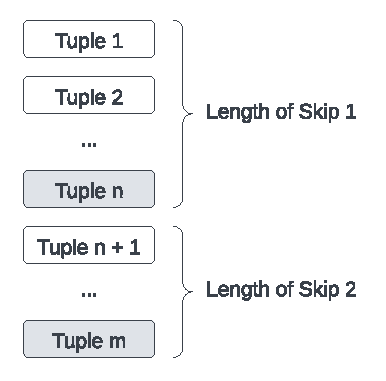
\includegraphics[height=5cm]{figure1.pdf}
            \caption{Example of two Skips with different lengths}
            \label{fig:skips}
        \end{figure}

        % Preallocation
        The length of a Skip is stored with some additional metadata in node. To ensure the constant use of memory it is necessary that the maximum amount of threads that can be used for inserting is known when the algorithm is initialized. In consequence, all nodes can be preallocated, one for every thread and one additional node as reserve. On benefit is that no more memory allocation is required at run time and that a pointer to a node can simply be an index into the node array.

        % Multithreaded nodes
        Hence, Skips are already stored in self contained nodes, these nodes can easily be distributed among multiple threads. Once a thread has received a Skip, the thread can process tuples independently and can use its own Skip to determine which tuples to add to the sample. After the thread has reached a sample tuple and the length of the Skip has reached zero the thread needs to acquire a new Skip. Only the generation and distribution of Skips needs to be synchronized.

        % Lifecycle of a skip
        One additional field that is stored in every node, is a successor pointer. This pointer can be used to arrange nodes in a singly linked list and therefore to keep track of the state of a node. There are three states a node can be in, initially all nodes are in the free list. The free list contains all nodes that are currently not in use and can be considered as a pool of nodes that can be reused to store a Skip. If a Skip should be generated a node needs to be allocated, thus it is removed from the free list and the data of the Skip can be stored in this node. All generated Skips are stored in the list of Skips (LoS). The LoS always contains at least one Skip, this is also the reason why an extra reserve node needs to be allocated. When a thread needs to acquire a new Skip, it can pop the first item of the LoS. However, if the LoS only contains on item the thread needs to generate a new Skip and added to the LoS again. Figure \ref{fig:lifecycle} visualizes all three states and the transitions between these states.
        \begin{figure}[H]
            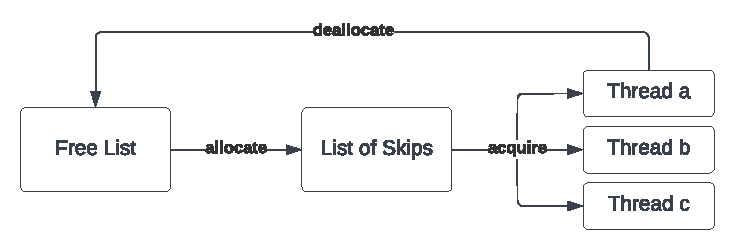
\includegraphics[height=2.8cm]{figure2.pdf}
            \caption{States of a node and the transitions between the states}
            \label{fig:lifecycle}
        \end{figure}

    \subsection{Inserting}
        % Description of the process
        Every thread receives an independent stream of tuples that should be inserted and therefore also sampled. The amount of tuples is unknown and each thread could stop receiving tuples at any moment. Every tuple  that the thread receives is inserted into the database and if the tuple is a sample tuple it is also added to the sample. To determine if a tuple is a sample tuple or not the thread needs to own a valid Skip. The Skip could be invalid if the length has reached zero. Therefore, if the thread currently does not own a valid Skip it needs to acquire a new one from the LoS. Once the thread owns a Skip it can use the length to determine whether the tuple is a sample tuple using the process described above. Figure \ref{fig:inserting} shows a flow diagram that visualizes this process.

        % Synchronization
        Only two steps require additional synchronization, first if a new Skip needs to be acquired and second if the tuple needs to be inserted into the sample. However, both of these steps are only executed if a tuple is inserted into the sample and therefore most of the time no extra overhead is introduced. The two steps that require synchronization are highlighted in gray in figure \ref{fig:inserting}.
        \begin{figure}[H]
            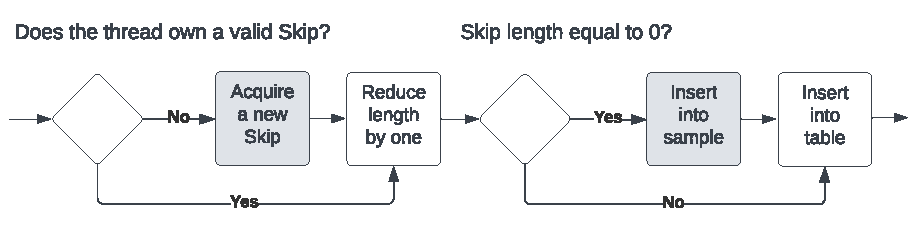
\includegraphics[height=2.2cm]{figure3.pdf}
            \caption{Flow diagram that shows the process of deciding whether a tuple is a sample tuple or not}
            \label{fig:inserting}
        \end{figure}        

        % Description of the sample
        All tuples that are added to the sample are inserted into a random position. In this phase of the algorithm the sample is always full and newly inserted tuples will override other tuples. But to ensure that two threads cannot write to the same row in the sample at the same time a very fine grained synchronization is applied. Every row has its own lock, therefore it is possible that two threads can write to different rows at the same time. In consequence the synchronization overhead for inserting into the sample is very low, because it is unlikely that a thread has to wait to acquire the lock for a row. 

        % Skip index
        Besides the actual tuple data the sample also stores the index of the Skip that inserted the tuple. The index of a Skip is stored in its metadata and can be used to determine the order in which the Skips where generated. Every time a new Skip is generated a counter is increased and its value can be used as the index for the current Skip.
        % Overwrite protection 
        The index can be used to ensure that older tuples cannot overwrite newer tuples. Thereupon when a new tuple should be inserted into the sample the Skip index of this tuple can be compared to the index in the sample and if the index of the tuple is smaller the insert will be rejected. This mechanism is important if there is for instance a slower thread that inserts into the database and a faster one. It could be the case that the faster one already inserted multiple tuples into the sample and if the slower thread later tries to insert a tuple into a row with a newer tuple, the slower thread would overwrite progress of the faster thread. Table \ref{tab:sample} visualizes an example sample table.
        \begin{table}[H]
            \begin{tabular}{| c | c | c | c|} 
                \hline
                Sample Index & Skip index & Lock & Tuple \\
                \hline
                \hline
                0 & 15 & 0 & DATA \\
                \hline
                1 & 42 & 0 & DATA \\
                \hline
                2 & 13 & 0 & DATA \\
                \hline
                ... & ... & ... & ... \\
                \hline
                $m - 1$ & 31 & 0 & DATA \\
                \hline
            \end{tabular}
            \vspace{5mm}
            \caption{Example of how a sample table could look like}
            \label{tab:sample}
        \end{table}

    \subsection{Ownership of Skips}
        % Recap
        In order to determine whether a tuple is a sample tuple or not a threads needs to own a Skip. To acquire a Skip the threads needs access the LoS. However, accessing the LoS requires synchronization and if the LoS contains only one Skip the thread needs to generate a new Skip.
        
        % How does the head pointer look like
        The free list and the LoS can be accessed using a head pointer. A pointer to a node is an index into the preallocated node are. Threads can only push a node or pop a node from a list. To ensure that no concurrent modifications can be meade to a list the head pointer is written with one atomic compare and swap operation. In order to detected changes between reading a node and make changes to the list a thread first needs to store the current pointer to a list. When the pointer changed in the meantime the compare and swap operation will fail. However, nodes are frequently added and removed to a list and it could be the case that the pointer was changed and then changed back to the original node. In this case the compare and swap operation would fail but the pointer was modified in the meantime. To address this problem the poin
        ter also contains a version besides the index. This pointer can be stored in 64 bit integer, hereby the first 32bit store the version and the rest stores the index. Figure \ref{fig:pointer} visualizes the layout of a pointer.
        \begin{figure}[H]
            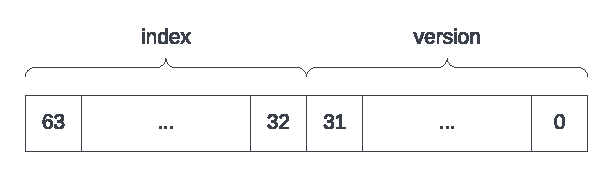
\includegraphics[height=2.2cm]{figure4.pdf}
            \caption{The structure of a head pointer}
            \label{fig:pointer}
        \end{figure}  

        % Actual acquiring
        The process of acquire a node from the LoS can be broken down into three steps. First the thread needs to read the head pointer and store the current value. Afterwards, the thread can use the index stored in the pointer to retrieve the node form the LoS. In the second step, the thread needs to generate the successor for the Skip stored in the node and lastly the thread tries to writes the successor into the head of the LoS. If the update succeeds the thread now owns a new Skip and the head of the LoS is set to the successor Skip. On the other hand, if the update fails, the thread needs to start over. However, in practice this is not a problem, because every time a thread fails to update the head, another thread successfully updated the head and therefore overall progress is guaranteed. Figure \ref{fig:acquire} shows the three steps necessary to acquire a Skip and the retry loop.
        \begin{figure}[H]
            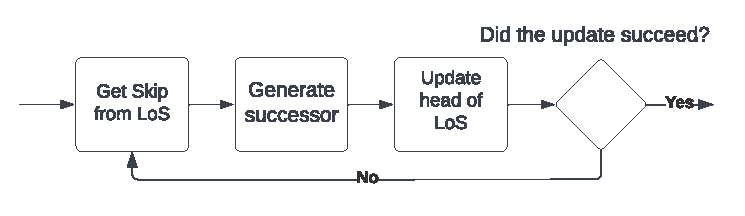
\includegraphics[height=2.4cm]{figure5.pdf}
            \caption{Flow diagram that shows the process of acquire a Skip from the LoS}
            \label{fig:acquire}
        \end{figure}

        % Generating the successor
        If the LoS only contains one node, the thread needs to generate a successor before takeing ownership of this node. In order to generate a Skip the thread needs to own a node, because nodes can only be modified when they are owned by a thread. It could be the case that the thread already owns a node from a previous iteration. On the other hand, if the thread does not own a node it needs to retrieve one from the free list. Using a node and the current Skip at the head of the LoS the thread can generate the successor. However, it could also be the case that the LoS contains more then one node and no successor needs to be generated. But if the thread already owns a node, it needs to deallocate this node. Because a thread cannot own more then one node. Deallocateing a node refers to inserting the node into the free list. To summarize, there a two cases where a thread needs to allocate or deallocate a node: 
        \begin{itemize}
            \item Allocate: If the thread does not own a node and the LoS only contains one node
            \item Deallocate: If the thread owns a node and the LoS contains more the one node
        \end{itemize}

        % Returning a skip
        Since an inserting thread could be terminated at any time it needs to be possible for a thread to return the Skip it is currently using. To return a Skip, the Skip needs to be added to the LoS.
        
    \section{Example}
        % Introduction to the example 
        The following example will illustrate hwo the algorithm could work with two inserting threads, $T0$ and $T1$. Figure \ref{fig:example} visualizes the state of all nodes and Skips used in this example. This example assumes that the sample as already been prefilled.
        \begin{figure}[H]
            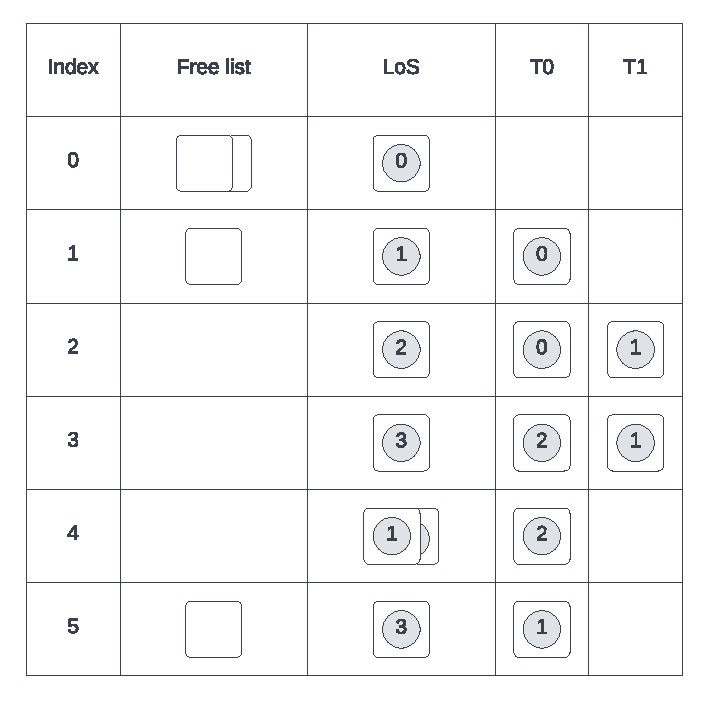
\includegraphics[height=8cm]{figure6.pdf}
            \caption{The state of every Skip and node for the example}
            \label{fig:example}
        \end{figure}

        % An example who the algorithm works (like the one in the OG)
        Initially all nodes are in the free list, except one node that contains the initial Skip (0). If $T0$ starts inserting it needs to acquire a Skip from the LoS. But because the LoS only contains one entry, $T0$ needs to generate a successor. However, $T0$ does not own a node and therefore it needs to retrieve one from the free list. Using this node and the initial Skip $T0$ can now generate the first Skip and swap it with the head of LoS. Afterwards $T0$ owns the initial Skip and the LoS contains the newly generated first Skip (1). When $T1$ also starts inserting it also needs to retrieve a Skip from the LoS. Since the LoS still contains just one Skip, $T1$ also needs to generate the second Skip and swap it with the head of the LoS (2). In the meantime $T0$ reach a sample tuple and needs a new Skip to continue inserting. The LoS only contains one element, but this time $T0$ already owns a node from the previous iteration. Therefore, $T0$ can use its node and the Skip from the LoS to generate the third Skip. $T0$ can now swap the newly generated Skip with the second Skip, to take ownership of the second Skip (3). In this example $T1$ is terminated before it reaches a sample tuple. In consequence $T1$ needs to return its Skip to the LoS. The LoS now contains two elements, Skip 1 that was previously owned by $T1$ and Skip 3 that was generated by $T0$ (4). At last $T0$ needs another Skip to continue inserting. This time $T0$ again owns a node from the previous iteration, but the LoS contains two elements. Therefore $T0$ does not need to generate a successor and can simply take ownership of the first Skip stored in the LoS. However, $T0$ cannot own two nodes and therefore $T0$ inserts the node of the previous Skip into the free list (5).

        This example contains both allocation and deallocation. $T0$ needs to allocate a node in step 1 and $T1$ needs to allocate a node in step 2. Because $T1$ returns its Skip, the LoS contains two Skips after Step 4. Therefore, $T0$ needs to deallocate its own node in Step 5.


    \section{Evaluation}
        % Are all requirements met
        % Tables from the OG
        This is the evaluation.

    \bibliographystyle{ACM-Reference-Format}
    \bibliography{sources}

\end{document}